\documentclass[11pt]{book}

% \def\class{122}
% \newcommand{\AllSections}[1]{\ifnum\class=0 #1 \fi}
% \newcommand{\DifferentialCalc}[1]{\ifnum\class=121 #1 \fi}
% \newcommand{\IntegralCalc}[1]{\ifnum\class=122 #1 \fi}
% \newcommand{\AcceleratedCalc}[1]{\ifnum\class=131 #1 \fi}
% \newcommand{\IntroMathModeling}[1]{\ifnum\class=141 #1 \fi}
% 


\setlength{\oddsidemargin}{0.1in}
\setlength{\evensidemargin}{0.1in}
\setlength{\textwidth}{6.5in}
\setlength{\topmargin}{.04in}
\setlength{\textheight}{8.2in}

%% AMS packages

\usepackage{amsmath,amsfonts,amssymb,amsthm,multicol}
\usepackage{tikz,pgfplots,xcolor}
\usetikzlibrary{arrows,shapes,petri,topaths}
\usepackage{tkz-berge}
\usetikzlibrary{decorations.pathmorphing}
\usepackage[framemethod=tikz]{mdframed}
\usepackage{boiboites}
%% other packages
% note that "epstopdf" is required for Mac users

\usepackage{graphics,epstopdf,fancyhdr,palatino}
\usepackage{makeidx}
\makeindex

% =============================================
% =============================================
% If you want to include the clicker questions directly in the text then turn this binary
% switch on (1).  Otherwise turn it off
% \def\EmbedClickers{0}
% \newcommand{\clicker}[1]{ \ifnum\EmbedClickers=1 \noindent {\bf Voting Questions}
% #1 \fi}
% 
% \newcommand{\voting}[1]{{\color{red} {\bf Voting Questions:} #1}}
% =============================================
% =============================================
\usepackage{hyperref} 
\hypersetup{colorlinks=true, linkcolor=blue,  anchorcolor=blue,  
citecolor=blue, filecolor=blue, menucolor=blue, pagecolor=blue,  
urlcolor=blue,pdftitle={ACmain}}

%% Packages to use the MathDesign _Charter_ font.

%\usepackage[T1]{fontenc}
%\usepackage[charter]{mathdesign}

%% Activities package

% Options to the activities package are: "bighints", "smallhints",
% "activitysolutions" (which are mutually exclusive; the last one listed is the
% one used) "exercisesolutions", and "authornotes".  If the option is there, then
% the corresponding environment is shown.

\usepackage{activities}

\lhead[\fancyplain{}{\thepage}]         {\fancyplain{}{\rightmark}}
\chead[\fancyplain{}{}]                 {\fancyplain{}{}}
\rhead[\fancyplain{}{\rightmark}]       {\fancyplain{\thepage}}

% \rfoot[\fancyplain{}{}] {\fancyplain{}{\scalebox{0.35}{\includegraphics{figures/CClicense.eps}} }} 

\cfoot[\fancyplain{\thepage}{}] {\fancyplain{\thepage}{}} 

\lfoot[ \fancyplain{ \scalebox{0.35}{\includegraphics{figures/CClicense.eps}}  }  { \scalebox{0.35}{\includegraphics{figures/CClicense.eps}}  } ] {\fancyplain{}{}}

\newcounter{cnt}
\newenvironment{numlist}{\begin{list}{(\arabic{cnt})}{\usecounter{cnt}
\setlength{\leftmargin}{.35 in}\setlength{\labelwidth}{.35 in}
\setlength{\itemsep}{10 pt}}}{\end{list}}

\newcounter{cnt4}
\newenvironment{numlist2}{\begin{list}{(\arabic{cnt4})}{\usecounter{cnt4}
\setlength{\leftmargin}{.5 in}\setlength{\labelwidth}{.25 in}
\setlength{\itemsep}{10 pt}}}{\end{list}}

\newcounter{cnt2}
\newenvironment{alphalist}{\vspace*{-3 pt}\begin{list}{(\alph{cnt2})}{\usecounter{cnt2}
\setlength{\leftmargin}{.5 in}\setlength{\labelwidth}{.25
in}\setlength{\itemsep}{5 pt}}}{\end{list}}

\newcounter{cnt3}
\newenvironment{alphalist2}{\vspace*{-3 pt}\begin{list}{(\alph{cnt3})}{\usecounter{cnt3}
\setlength{\leftmargin}{.25 in}\setlength{\labelwidth}{.25
in}\setlength{\itemsep}{5 pt}}}{\end{list}}

\newcounter{cnt5}
\newenvironment{thmlist}{\vspace*{-3 pt}\begin{list}{{\em (\roman{cnt5})}}{\usecounter{cnt5}
\setlength{\leftmargin}{.5 in}\setlength{\labelwidth}{.25
in}\setlength{\itemsep}{3 pt}}}{\end{list}}

%\newcommand{\lint}{\raisebox{-.14 in}{\underline{\hspace*{.7 ex}}}
%\hspace*{-1 ex} \int}

%\newcommand{\uint}{\hspace*{1.5 ex} \raisebox{.296 in}{\underline{\hspace*{.7 ex}}}
%\hspace*{-2.3 ex} \int}

\setlength{\parskip}{5 pt}

\newcounter{lastenum}
\newcommand{\saveCount}{\setcounter{lastenum}{\value{enumi}}}
\newcommand{\restoreCount}{\setcounter{enumi}{\value{lastenum}}}

\newcommand{\be}{\begin{numlist}}
\newcommand{\ee}{\end{numlist}}
\newcommand{\bei}{\begin{numlist2}}
\newcommand{\eei}{\end{numlist2}}
\newcommand{\ba}{\begin{alphalist}}
\newcommand{\ea}{\end{alphalist}}
\newcommand{\bal}{\begin{alphalist2}}
\newcommand{\eal}{\end{alphalist2}}
\newcommand{\bi}{\begin{itemize}}
\newcommand{\ei}{\end{itemize}}
\newcommand{\btl}{\begin{thmlist}}
\newcommand{\etl}{\end{thmlist}}

\newcommand{\bpm}{\begin{pmatrix}}
\newcommand{\epm}{\end{pmatrix}}
\newcommand{\bolda}{\boldsymbol{a}}
\newcommand{\boldx}{\boldsymbol{x}}
\newcommand{\boldy}{\boldsymbol{y}}
\newcommand{\boldb}{\boldsymbol{b}}
\newcommand{\boldv}{\boldsymbol{v}}
\newcommand{\boldu}{\boldsymbol{u}}
\newcommand{\bx}{\boldsymbol{x}}
\newcommand{\by}{\boldsymbol{y}}
\newcommand{\bu}{\boldsymbol{u}}
\newcommand{\bv}{\boldsymbol{v}}
\newcommand{\bd}{\boldsymbol{d}}

% theorem-like environments
\theoremstyle{definition}
\newtheorem{pa}{Preview Activity}[chapter]
\newtheorem{example}{Example}[chapter]
% \newtheorem{definition}{Definition}[chapter]




\newcounter{definition}
% \stepcounter{definition}
\renewcommand{\thedefinition}{\thechapter.\arabic{definition}}
% \mdfdefinestyle{definition}{
%     backgroundcolor=green!10, linecolor=green, outerlinewidth=1pt, roundcorner=5mm,
%     skipbelow=\baselineskip,
%     frametitle=\mbox{},
% }
% \newmdenv[%
%     style=definition,
%     settings={\global\refstepcounter{definition}},
%     frametitlefont={\bfseries {\large Definition}~\thedefinition\quad},
% ]{definition}
\newboxedtheorem[boxcolor=green,
    background=green!10,
    titlebackground=green!10,
titleboxcolor=black]
{definition}{Definition}{definition}



\mdfdefinestyle{callout}{
    backgroundcolor=yellow!30, linecolor=red, outerlinewidth=1pt, roundcorner=5mm,
    skipbelow=\baselineskip,
    frametitle=\mbox{},
}
\newmdenv[%
    style=callout,
%     settings={\global\refstepcounter{definition}},
%     frametitlefont={\bfseries {\large Definition}~\thedefinition\quad},
]{callout}

\newcounter{corollary}
% \stepcounter{corollary}
\renewcommand{\thecorollary}{\thechapter.\arabic{corollary}}
\newboxedtheorem[boxcolor=red, 
    background=red!15, 
    titlebackground=red!5,
titleboxcolor = black]
{corollary}{Corollary}{corollary}



\newcounter{theorem}
% \stepcounter{theorem}
\renewcommand{\thetheorem}{\thechapter.\arabic{theorem}}
% \mdfdefinestyle{theorem}{
%     backgroundcolor=blue!10, linecolor=blue, outerlinewidth=1pt, roundcorner=5mm,
%     skipbelow=\baselineskip,
%     frametitle=\mbox{},
% }
% \newmdenv[%
%     style=theorem,
%     settings={\global\refstepcounter{theorem}},
%     frametitlefont={\bfseries {\large Theorem}~\thetheorem\quad},
% ]{theorem}
\newboxedtheorem[boxcolor=blue,
    background=blue!10,
    titlebackground=blue!10,
titleboxcolor=black]
{theorem}{Theorem}{theorem}




\newcommand{\bex}{\begin{center}\underline{\hspace{5.0in}}\end{center} \begin{example}}
\newcommand{\eex}{\end{example} \noindent{\bf Solution.}~~}
\newcommand{\afterex}{\begin{center}\underline{\hspace{5.0in}}\end{center}}
\newcommand{\afterexercises}{\nin \hrulefill \vfill \ \newpage}

% my commands

\newcommand{\ds}{\ensuremath{\displaystyle}}
\newcommand{\nin}{\noindent}
\newcommand{\tr}{\vspace*{0.5in}}
\newcommand{\lr}{\vspace*{1.0in}}
\newcommand{\mr}{\vspace*{2.0in}}
\newcommand{\br}{\vspace*{3.0in}}
\newcommand{\afterpa}{\hfill $\bowtie$}
\newcommand{\aftera}{\hfill $\lhd$}

\newcommand\T{\rule{0pt}{2.6ex}}
\newcommand\B{\rule[-1.2ex]{0pt}{0pt}}

\newcommand{\vs}{\vspace*{0.1in}}
\newcommand{\solution}{\noindent{\bf Solution.}}

\newenvironment{goals}{ \vspace*{7 pt}{\large \textbf{Motivating Questions}} \vspace*{-6 pt} \\ ~\hrule~ \vspace*{2 pt}

 {\em In this section, we strive to understand the ideas generated by the following important questions:}
\vspace*{-5 pt} \\ ~\hrule~ \vspace*{-3 pt}
\begin{list}{\labelitemi}{\leftmargin=1.25em}
\setlength{\itemsep}{3 pt}}{ \end{list} \vspace*{-2 pt}}

\newenvironment{summary}{ %\vspace*{7 pt}
\nin{\large \textbf{Summary}} \vspace*{-6 pt} \\ ~\hrule~ \vspace*{2 pt}
\nin{\em \hspace*{-10pt} In this section, we encountered the following important ideas:}
\vspace*{-9 pt} \\ ~\hrule~ \vspace*{-3 pt}
\begin{list}{\labelitemi}{\leftmargin=1.25em}
\setlength{\itemsep}{3 pt}}{ \end{list} \vspace*{-2 pt}}

\pagestyle{fancyplain}

% the following inclusion is for the figure pertaining to matrix multiplication in chapter
% 10.
\usepackage[utf8]{inputenc}
\usepackage[upright]{fourier}
% \usepackage{tikz}
\usetikzlibrary{matrix,arrows,decorations.pathmorphing}

\newcommand{\myunit}{1 cm}
\tikzset{
    node style sp/.style={draw,circle,minimum size=\myunit},
    node style ge/.style={circle,minimum size=\myunit},
    arrow style mul/.style={draw,sloped,midway,fill=white},
    arrow style plus/.style={midway,sloped,fill=white},
}


%TABLE/GRAPH ON ONE LINE COMMANDS
%\begin{figure}[h]
%\centering
%\begin{tabular}{cc}
%	\raisebox{.75in}{\begin{tabular}[b]{c|c} $x$ & $y$ \\ \hline a & b \\ c & d \\ e & f  \end{tabular} } &	
%	\hspace{1in} \includegraphics[2in,2in]{c:/mth310/project/Hamilton.bmp} 
%\end{tabular}
%\caption{{\scriptsize Table and graph for $f$.}}
%\end{figure}

%%%%%%%%%%%%%%%%%%%%%%%%%%%%%%%%%%%%%%%%%%%%%%%%%%%%

\title{Active Calculus \\ Activities Book \\ \vspace{0.1in} \scalebox{0.75}{\includegraphics{figures/CClicense.eps}}}
% \title{Active Calculus \\ \vspace{0.1in} \scalebox{0.75}{\includegraphics{figures/CClicense.eps}}}
%\date{\today}
\author{
Active Calculus: Matt Boelkins, Lead Author and Editor \\ Department of Mathematics \\ Grand Valley State University \\ 
\texttt{boelkinm@gvsu.edu} \\ 
\href{http://faculty.gvsu.edu/boelkinm/}{\texttt{http://faculty.gvsu.edu/boelkinm/}}\\
David Austin, Contributing Author \\
\href{http://merganser.math.gvsu.edu/david/}{\texttt{http://merganser.math.gvsu.edu/david/}} \\
Steven Schlicker, Contributing Author \\
\href{http://faculty.gvsu.edu/schlicks/}{\texttt{http://faculty.gvsu.edu/schlicks/}} \\
\vspace{0.5in} \\
Carroll College: Eric Sullivan, Contributing Author and Editor \\ \texttt{esullivan@carroll.edu} \\
\href{http://www.carroll.edu/esullivan}{\texttt{http://www.carroll.edu/esullivan}}  
} 

\date{Last Updated: \today}

%\includeonly{6.chap}

\begin{document}
% \frontmatter
% \dominitoc
\maketitle
\tableofcontents



% \setcounter{chapter}{-1} % this sets the counter back so that the prelims are ``chapter 0''
% \input{0.preface}
% 
\mainmatter

\chapter{Preliminaries}\label{C:0}

\section{Functions, Slope, and Lines} \label{S:0.1.Functions}

\begin{pa} \label{PA:0.1}
    This is the first Preview Activity in this text.  Your job for this activity is to get
    to know the textbook.
    \ba
    \item Where is the full textbook stored?  Find it and save a copy to your computer.
    \item What chapters of this text are you going to cover this semester.  Have a look at
        your syllabus!
%     \item There are a few appendices in the textbook.  What are they and 
%         where are they?
    \item What are the differences between Preview Activities, Activities, Examples,
        Exercises, Voting Questions, and WeBWork?  Which ones should you do before class,
        which ones will you likely do during class, and which ones should you be doing
        after class?
    \item What materials in this text would you use to prepare for an exam and where do
        you find them?
    \item What should you bring to class every day?
    \ea
\end{pa} \afterpa

\newpage
\begin{activity}\label{A:0.1.1}
The graph of a function f is shown below. 

\begin{center}
    \begin{tikzpicture}
        \begin{axis}[axis lines=center, xmin=-1, xmax=5, ymin=-3, ymax=10, grid,
            xlabel={$x$}, ylabel={$y$}, title={$f(x)$}]
            \addplot[smooth, blue, very thick, domain=-1:5] {0.5*(x+1)*(x-2)*(x-4)};
        \end{axis}
    \end{tikzpicture}
\end{center}

\ba
\item What are the domain and range of $f$?
\item What are  $f(-1)$, $f(1)$, $f(3)$, $f(5)$?
\ea

\end{activity}\aftera

\newpage
\begin{activity}\label{A:0.1.2}
Find the equation of the line with the given information.
\ba
\item The line goes through the points $(-2,5)$ and $(10,-1)$.
\item The slope of the line is $3/5$ and it goes through the point $(2,3)$.
\item The $y$-intercept of the line is $(0,-1)$ and the slope is $-2/3$.
\ea

\end{activity}
\begin{smallhint}
   \ba
        \item Recall that $m = \frac{\Delta y}{\Delta x}$ and use the point slope form of
            the line.
        \item You are given a slope and a point.  Which form of the line should you use?
        \item You are given a slope and the $y$ intercept.  Which form of the line should
            you use?
   \ea
\end{smallhint}
\begin{bighint}
   \ba
        \item The slope is $m = \frac{\Delta y}{\Delta x} = \frac{5-(-1)}{(-2)-10} =
            \frac{6}{-12} = -\frac{1}{2}$.  Now use the point-slope form of the line.
        \item The point-slope form of the line is best here.
        \item The slope-intercept form of the line is best here.
   \ea
\end{bighint}
\begin{activitySolution}
   \ba
        \item The slope is $m = \frac{\Delta y}{\Delta x} = \frac{5-(-1)}{(-2)-10} =
            \frac{6}{-12} = -\frac{1}{2}$.  Hence,
            \[ y - 5 = -\frac{1}{2} \left( x-(-2) \right) \]
            which can be rewritten as
            \[ y = -\frac{1}{2} \left( x+2 \right) + 5. \]
        \item Using the point-slope form of the line we get
            \[ y - 3 = \frac{3}{5} \left( x-2 \right) \]
            which can be rearranged to 
            \[ y = \frac{3}{5} \left( x-2 \right) + 3. \]
        \item Using the slope-intercept form of the line we get
            \[ y = -\frac{2}{3} x - 1. \]
   \ea
\end{activitySolution}
\aftera

\newpage
\begin{activity}\label{A:0.1.3}
A simulation shows lifetime peptic ulcer rates per 100 population for different
family incomes as given in the following table.

\begin{minipage}{0.3\columnwidth}
    \begin{center}
    \begin{tabular}{|c|c|}
        \hline
        Income  & Ulcer Rate\\
        \hline \hline
        \$4000  & 14.1\\
        \$8000  & 13.4\\
        \$12000 &12.5\\
        \$16000 &12\\
        \$20000 &12.4\\
        \$24000 &11.6\\
        \$28000 &10.8\\
        \$32000 &10.3\\
        \$36000 &10.4\\
        \$40000 & 9.6\\
        \$44000 & 9.2\\
        \$48000 & 8.8\\
        \$52000 & 8.5\\
        \$56000 & 8.4\\
        \$60000 & 8.2\\ \hline
    \end{tabular}
\end{center}
\end{minipage}
\begin{minipage}{0.3\columnwidth}
    \begin{center}
        \begin{tikzpicture}
            \begin{axis}[xmin=0, xmax=60, ymin=0, ymax=16, xlabel={Income (thousands of
                dollars)}, ylabel={Ulcer Rate}, grid,
            xtick={4,8,12,16,20,24,28,32,36,40,44,48,52,56,60}, xscale=1.5,
        ytick={2,4,6,8,10,12,14,16}]
                \addplot[smooth] {0*x};
            \end{axis}
        \end{tikzpicture}
    \end{center}
\end{minipage}

This data does not represent a straight line, but it is close.
\ba 
\item Just by doing simple arithmetic, how can you tell the function is not a straight
    line?

\item Make a scatter plot of the data.  Do you think a linear model can be a good
    approximation?  Why or why not?

\item Use just the first and the last data points, what is the equation of the straight
    line that these two points determine?  Graph this equation.

\item Using the model in part (c), estimate the ulcer rate for an income of \$26000.

\item Using the model in part (c), how likely is someone with an income of \$100,000 will
    suffer from peptic ulcers?  Note your answer will be a percent and remember that the
    ulcer rate is given per 100 people of population.

\item Do you think it would be reasonable to apply this model to a person with an income
    of \$200,000?  Why or why not?
\ea
\end{activity}
\begin{smallhint}
   \ba
        \item Recall what we know about slope on a linear function.
        \item The data do not fall on one line, but are they close?
        \item It might be best to find slope first
        \item Once you have the linear function you can use it to make predictions.
        \item 
        \item
   \ea
\end{smallhint}
\begin{bighint}
   \ba
        \item
        \item
        \item
        \item
        \item
        \item
   \ea
\end{bighint}
\begin{activitySolution}
   \ba
        \item 
        \item
        \item
        \item
        \item
        \item
   \ea
\end{activitySolution}
\aftera

\newpage
\begin{activity}\label{A:0.1.4}
Write the equation of the line with the given information.
\ba
\item Write the equation of a line parallel to the line $y=\frac{1}{2}x+3$ passing through
    the point $(3,4)$.
\item Write the equation of a line perpendicular to the line $y=\frac{1}{2}x + 3$ passing
    through the point $(3,4)$.
\item Write the equation of a line with $y$-intercept $(0,-3)$ that is perpendicular to
    the line $y=-3x-1$.
\ea
\end{activity}
\begin{smallhint}
    \ba
        \item What is the slope of the line that you're given and which form of a linear
            function would be most convenient?
        \item What is the slope of the line that you're given and which form of a linear
            function would be most convenient?
        \item You are given the $y$-intercept.  Why is that a special case?
    \ea
\end{smallhint}
\begin{bighint}
    \ba
        \item The slope should be the same since the lines are parallel.
        \item The slope should be the opposite reciprocal since the lines are
            perpendicular.
        \item The slope should be the opposite reciprocal since the lines are
            perpendicular.
    \ea
\end{bighint}
\begin{activitySolution}
    \ba
        \item The slope is $m = \frac{1}{2}$ and you have a point so use the point-slope
            form of the line to get
            \[ y - 4 = \frac{1}{2} \left( x-3 \right). \]
            Solving for $y$ we get 
            \[ y = \frac{1}{2} \left( x-3 \right) + 4. \]
        \item The slope is $m = -2$ and we have a point so use the point-slope form of the
            line to get
            \[ y - 4 = -2 (x-3). \]
            Solving for $y$ we get 
            \[ y = -2(x-3) + 4. \]
        \item The slope is $m = \frac{1}{3}$ and since we have the $y$-intercept we know
            that the slope-intercept for the line is the proper choice.  Hence,
            \[ y = \frac{1}{3} x - 3. \]
    \ea
\end{activitySolution}



\aftera

\newpage
\begin{activity}\label{A:0.1.5}
    Classify each of the following as an expression, equation, or a function.  For each
    function, classify it as either linear or non-linear.  Finally, for each linear
    function find the slope and $y$-intercept.
    \ba
    \item $y=6y-3$
    \item $y=6x-3$
    \item $6x-3$
    \item $-4y+2x+8=0$
    \item $12x=6y+4$
    \item $12x=6y^2+4$
    \item $\sqrt{x+2}$
    \item $y=\sqrt{x+2}$
    \item $x=\sqrt{x+2}$
    \item $x^2+2x-3$
    \item $x+2x-3=9$
    \ea

\end{activity}\aftera

\newpage
\subsection*{Voting Questions}
\renewcommand{\labelenumi}{\thesection.\arabic{enumi}}
\begin{enumerate}
        \input{clicker/SVC.01.01.001.tex}
        \teacher{\input{clicker/SVC.01.01.001C.tex}}
        \input{clicker/SVC.01.01.002.tex}
        \teacher{\input{clicker/SVC.01.01.002C.tex}}
        \input{clicker/SVC.01.01.003.tex}
        \teacher{\input{clicker/SVC.01.01.003C.tex}}
        \input{clicker/SVC.01.01.004.tex}
        \teacher{\input{clicker/SVC.01.01.004C.tex}}
        \input{clicker/SVC.01.01.005.tex}
        \teacher{\input{clicker/SVC.01.01.005C.tex}}
        \input{clicker/SVC.01.01.010.tex}
        \teacher{\input{clicker/SVC.01.01.010C.tex}}
        \input{clicker/SVC.01.01.011.tex}
        \teacher{\input{clicker/SVC.01.01.011C.tex}}
        \input{clicker/SVC.01.01.012.tex}
        \teacher{\input{clicker/SVC.01.01.012C.tex}}
        \input{clicker/SVC.01.01.013.tex}
        \teacher{\input{clicker/SVC.01.01.013C.tex}}
        \input{clicker/SVC.01.01.014.tex}
        \teacher{\input{clicker/SVC.01.01.014C.tex}}
        \input{clicker/SVC.01.01.015.tex}
        \teacher{\input{clicker/SVC.01.01.015C.tex}}
        \input{clicker/SVC.01.01.020.tex}
        \teacher{\input{clicker/SVC.01.01.020C.tex}}
        \input{clicker/SVC.01.01.030.tex}
        \teacher{\input{clicker/SVC.01.01.030C.tex}}
        \input{clicker/SVC.01.01.040.tex}
        \teacher{\input{clicker/SVC.01.01.040C.tex}}
        \input{clicker/SVC.01.01.050.tex}
        \teacher{\input{clicker/SVC.01.01.050C.tex}}
        \input{clicker/SVC.01.01.051.tex}
        \teacher{\input{clicker/SVC.01.01.051C.tex}}
        \input{clicker/SVC.01.01.052.tex}
        \teacher{\input{clicker/SVC.01.01.052C.tex}}
        \input{clicker/SVC.01.01.060.tex}
        \teacher{\input{clicker/SVC.01.01.060C.tex}}
        \input{clicker/SVC.01.01.070.tex}
        \teacher{\input{clicker/SVC.01.01.070C.tex}}
        \input{clicker/SVC.01.01.080.tex}
        \teacher{\input{clicker/SVC.01.01.080C.tex}}
        \input{clicker/SVC.01.01.090.tex}
        \teacher{\input{clicker/SVC.01.01.090C.tex}}
        \input{clicker/SVC.01.01.100.tex}
        \teacher{\input{clicker/SVC.01.01.100C.tex}}
        \input{clicker/SVC.01.01.110.tex}
        \teacher{\input{clicker/SVC.01.01.110C.tex}}
        \input{clicker/SVC.01.01.120.tex}
        \teacher{\input{clicker/SVC.01.01.120C.tex}}
        \input{clicker/SVC.01.01.130.tex}
        \teacher{\input{clicker/SVC.01.01.130C.tex}}
        \input{clicker/SVC.01.01.140.tex}
        \teacher{\input{clicker/SVC.01.01.140C.tex}}
        \input{clicker/SVC.01.01.150.tex}
        \teacher{\input{clicker/SVC.01.01.150C.tex}}
        \input{clicker/SVC.01.01.160.tex}
        \teacher{\input{clicker/SVC.01.01.160C.tex}}
        \input{clicker/SVC.01.01.170.tex}
        \teacher{\input{clicker/SVC.01.01.170C.tex}}
        \input{clicker/SVC.01.01.180.tex}
        \teacher{\input{clicker/SVC.01.01.180C.tex}}
        \input{clicker/SVC.01.01.190.tex}
        \teacher{\input{clicker/SVC.01.01.190C.tex}}
        \input{clicker/SVC.01.01.200.tex}
        \teacher{\input{clicker/SVC.01.01.200C.tex}}
        \input{clicker/SVC.01.01.210.tex}
        \teacher{\input{clicker/SVC.01.01.210C.tex}}
\end{enumerate}
\renewcommand{\labelenumi}{\arabic{enumi}}

\newpage

\section{Exponential Functions} \label{S:0.2.Exponentials}

\begin{pa} \label{PA:0.2}
Suppose that the populations of two towns are both growing over time.  The town of
Exponentia is growing at a rate of 2\% per year, and the town of Lineola is growing at a
rate of 100 people per year.  In 2014, both of the towns have 2,000 people.
\ba
    \item Complete the table for the population of each of these towns over the next
        several years.
        \begin{center}
            \begin{tabular}[h!]{|c|c|c|c|c|c|c|c|c|c|c|c|}
                \hline
                & 2014 & 2015 & 2016 & 2017 & 2018 & 2019 & 2020 & 2021 & 2022 \\ \hline
                Exponentia & 2000 & & & & & & & & \\ \hline
                Lineola &  2000 & & & & & & & & \\ \hline
            \end{tabular}
        \end{center}
    \item Write a linear function for the population of Lineola. Interpret the slope in
        the context of this problem.
    \item The ratio of successive populations for Exponentia should be equal.  For
        example, dividing the population in 2015 by that of 2014 should give the same
        ratio as when the population from 2016 is divided by the population of 2015.  Find
        this ratio.  How is this ratio related to the 2\% growth rate?
    \item Based on your data from part (a) and your ratio in part (c), write a function
        for the population of Exponentia.
    \item When will the population of Exponentia exceed that of Lineola?
\ea
\end{pa} \afterpa

\newpage
\begin{activity}\label{A:0.2.1}
    Consider the exponential functions plotted in Figure \ref{F:0.2.Act1}
    \ba
        \item Which of the functions have common ratio $r > 1$?
        \item Which of the functions have common ratio $0<r< 1$?
        \item Rank each of the functions in order from largest to smallest $r$ value.
    \ea
    \begin{figure}[h!]
        \begin{center}
%             \begin{tikzpicture}
%                 \begin{axis}[axis lines=center, xlabel={$x$}, ylabel={$y$}, xmin=-3, xmax=3,
%                     ymin=-1, ymax=5, domain=-3:3,legend pos=outer north east]
%                     \addplot[smooth, blue, very thick] {2^x};
%                     \addlegendentry{$f(x)$};
%                     \addplot[smooth, red, very thick, dashed] {3^x};
%                     \addlegendentry{$g(x)$};
%                     \addplot[smooth, green!50!black, very thick, dotted] {1.5^x};
%                     \addlegendentry{$h(x)$};
%                     \addplot[smooth, black, very thick, dashdotted] {(0.5)^x};
%                     \addlegendentry{$k(x)$};
%                     \addplot[smooth, cyan, very thick, densely dotted] {(0.9)^x};
%                     \addlegendentry{$m(x)$};
%                 \end{axis}
%             \end{tikzpicture}
            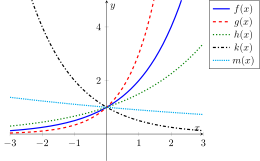
\includegraphics[width=0.6\columnwidth]{figures/0-2-figAct1.pdf}
        \end{center}
        \caption{Exponential growth and decay functions} \label{F:0.2.Act1}
    \end{figure}
\end{activity}
\begin{smallhint}
   \ba
        \item If the common ratio is larger than 1 what will happen to the $y$ values?
            For example, if the common ratio were 2 and we start with 5 then what would
            the next value be?
        \item If the comon ratio is less than 1 what will happen to the $y$ values?
        \item Do some experimentation to determine which ones will be steeper or less
            steep.
   \ea
\end{smallhint}
\begin{bighint}
   \ba
        \item If we start with 5 and the common ratio is 2 then the next value would be
            10, then 20, then 40, etc.
        \item If we start with 5 and the common ratio is $1/2$ then the next value would
            be $5/2$, then $5/4$, then $5/8$, etc.
        \item The exponential growth functions that grow fastest have the larger common
            ratio.
   \ea
\end{bighint}
\begin{activitySolution}
   \ba
        \item blue, red, dark green
        \item cyan and black
        \item blue is $y = 2^x$, red is $y = 3^x$, dark green is $y=1.5^x$, cyan is
            $y=0.9^x$, and black is $y=0.5^x$.
   \ea
\end{activitySolution}

\aftera

\newpage
\begin{activity}\label{A:0.2.2}
    A sample of $Ni^{56}$ has a half-life of 6.4 days.  Assume that there are 30 grams
    present initially.
    \ba
        \item Write a function describing the number of grams of $Ni^{56}$ present as a
            function of time.  Check your function based on the fact that in 6.4 days
            there should be 50\% remaining.
        \item What percent of the substance is present after 1 day?
        \item What percent of the substance is present after 10 days?
    \ea
\end{activity}
\begin{smallhint}
   \ba
        \item The growth rate should be $1/2$.
        \item Figure out how much is there after 1 day and divide by the original amount.
        \item Figure out how much is there after 10 days and divide by the original amount.
   \ea
\end{smallhint}
\begin{bighint}
   \ba
        \item When you substitute $6.4$ for the time you should have decayed by exactly
            half.
        \item Figure out how much is there after 1 day and divide by the original amount.
        \item Figure out how much is there after 10 days and divide by the original amount.
   \ea
\end{bighint}
\begin{activitySolution}
   \ba
        \item $A(t) = 30 \left( \frac{1}{2}  \right)^{t/6.4}$
        \item $A(1) =  30 \left( \frac{1}{2}  \right)^{1/6.4} \approx 26.9206$ so the
            percent that remains is just shy of 90\%.
        \item $A(10) =  30 \left( \frac{1}{2}  \right)^{10/6.4} \approx 10.1569$ so the
            percent that remains is about 33.9\%.
   \ea
\end{activitySolution}

\aftera

\newpage
\begin{activity}\label{A:0.2.3}%\cite[p.9]{nonlinear}
    Uncontrolled geometric growth of the bacterium {\it Escherichia coli (E. Coli)} is the
    theme of the following quote taken from the best-selling author Michael Crichton's
    science fiction thriller, {\it The Andromeda Strain:}
    \begin{quote}
        ``The mathematics of uncontrolled growth are frightening.  A single cell of the
        bacterium E. coli would, under ideal circumstances, divide every twenty minutes.
        That is not particularly disturbing until you think about it, but the fact is that
        that bacteria multiply geometrically: one becomes two, two become four, four
        become eight, and so on.  In this way it can be shown that in a single day, one
        cell of E. coli could produce a super-colony equal in size and weight to the
        entire planet Earth.''
    \end{quote}
    \ba
        \item Write an equation for the number of E. coli cells present if a single cell
            of E. coli divides every 20 minutes. 
        \item How many E. coli would there be at the end of 24 hours?
        \item The mass of an E. coli bacterium is $1.7 \times 10^{-12}$ grams, while the
            mass of the Earth is $6.0 \times 10^{27}$ grams.  Is Michael Crichton's claim
            accurate?  Approximate the number of hours we should have allowed for this
            statement to be correct?
    \ea
\end{activity}
\begin{smallhint}
   \ba
    \item What is the common ratio?
    \item Be sure to get your units correct.
    \item You might want to tackle this problem graphically.
   \ea
\end{smallhint}
\begin{bighint}
   \ba
    \item The common ratio is 2.
    \item If you have the units correct you should be substituting 1,440 minutes.
    \item You can do some algebra on your equation from part (a) to make your work easier.
   \ea
\end{bighint}
\begin{activitySolution}
   \ba
    \item $P(t) = P_0 \cdot 2^{t/20}$ where $t$ is measured in minutes.
    \item Assuming that $P_0 = 1$, $P(1440) = 2^{1440/20} \approx 4.72 \times 10^{21}$.
    \item 
        \begin{flalign*}
            6.0 \times 10^{27} &= 1.7 \times 10^{-12} \cdot 1 \cdot 2^{t/20} \\
            3.529 \times 10^{39} &= 2^{t/20} \\
            \log_2\left( 3.529 \times 10^{39} \right) &= \frac{t}{20} \\
            20 \log_2\left( 3.529 \times 10^{39} \right) &= t \\
            &\approx 2627.5 \text{ minutes}
        \end{flalign*}<++>
   \ea
\end{activitySolution}

\aftera

\newpage
% \begin{activity}\label{A:0.2.3}
The quantity, $Q$, of a drug in a patient's body at time $t$ is represented for positive
constants $S$ and $k$ by the function $Q(t) = S(1-e^{-kt})$. 
\ba
\item For $t \ge 0$ describe how $Q(t)$ changes with time.
\item Assuming that $S = 5$, use a graphing utility to make a sketch of $Q(t)$ with
    various values of $k$.  Use the left-hand side of Figure \ref{F:0.2.Act3} to organize
    your plots.  Interpret the value of $k$ in the context of this problem.
\item Now assume that $k=0.5$ and use a graphing utility to make a sketch of $Q(t)$ with
    various values of $S$.  Use the right-hand side of Figure \ref{F:0.2.Act3} to organize
    your plots.  Interpret the value of $S$ in the context of this problem.
\ea
\begin{figure}[h!]
    \begin{center}
        \begin{tikzpicture}
            \begin{axis}[axis lines=center,xlabel={$t$}, ylabel={$Q$}, xmin=0, ymin=0, xmax=6,
                ymax=10, grid, title={$Q(t)$ with $S=5$}]
                \addplot[smooth] {0*x};
            \end{axis}
        \end{tikzpicture}
        \begin{tikzpicture}
            \begin{axis}[axis lines=center,xlabel={$t$}, ylabel={$Q$}, xmin=0, ymin=0, xmax=6,
                ymax=10, grid, title={$Q(t)$ with $k=0.5$}]
                \addplot[smooth] {0*x};
            \end{axis}
        \end{tikzpicture}
    \end{center}
    \caption{Plot for Activity \ref{A:0.2.3}}
    \label{F:0.2.Act3}
\end{figure}
\end{activity}\aftera

% \newpage
\subsection*{Voting Questions}
\renewcommand{\labelenumi}{\thesection.\arabic{enumi}}
\begin{enumerate}
        \input{clicker/SVC.01.02.103.tex}
        \teacher{\input{clicker/SVC.01.02.103C.tex}}
        \input{clicker/SVC.01.02.104.tex}
        \teacher{\input{clicker/SVC.01.02.104C.tex}}
        \input{clicker/SVC.01.02.105.tex}
        \teacher{\input{clicker/SVC.01.02.105C.tex}}
        \input{clicker/SVC.01.02.106.tex}
        \teacher{\input{clicker/SVC.01.02.106C.tex}}
\end{enumerate}
\renewcommand{\labelenumi}{\arabic{enumi}}

\newpage

\section{Transformations of Functions} \label{S:0.3.NewFromOld}

\begin{pa} \label{PA:0.3}
The goal of this activity is to explore and experiment with the function
\[ F(x) = Af(B(x-C))+D. \]
The values of $A$, $B$, $C$, and $D$ are constants and the function $f(x)$ will be
henceforth called the {\it parent function}.  To facilitate this exploration, use the
applet located at \\
\href{http://www.geogebratube.org/student/m93018}{http://www.geogebratube.org/student/m93018}.
\ba
    \item Let's start with a simple parent function: $f(x) = x^2$.
        \bei
            \item Fix $B=1$, $C=0$, and $D=0$.  Write a sentence or two describing the
                action of $A$ on the function $F(x)$.
            \item Fix $A=1$, $B=1$, and $D=0$.  Write a sentence of two describing the
                action of $C$ on the function $F(x)$.
            \item Fix $A=1$, $B=1$, and $C=0$.  Write a sentence of two describing the
                action of $D$ on the function $F(x)$.
            \item Fix $A=1$, $C=0$, and $D=0$.  Write a sentence of two describing the
                action of $B$ on the function $F(x)$.
        \eei
    \item In part (a) you have made conjectures about what $A$, $B$, $C$, and $D$ do to a
        parent function graphically.  Test your conjectures with the functions $f(x) =
        |x|$ (typed \texttt{abs(x)}), $f(x) = x^3$, $f(x) = \sin(x)$, $f(x) = e^x$ (typed
        \texttt{exp(x)}), and any other function you find interesting. 
\ea
\end{pa} \afterpa

\newpage
\begin{activity}\label{A:0.3.1}
    Consider the function $f(x)$ displayed in Figure \ref{F:0.3.Act1}.
    \ba
        \item Plot $g(x) = -f(x)$ and $h(x) = f(x)-1$.
        \item Define the function $k(x) = -f(x)-1$.  Does it matter which order you
            complete the tranformations from part (a) to result in $k(x)$?  Plot the
            functions resulting from doing the two transformation in part (a) in opposite
            orders.  Which of these functions is $k(x)$?
    \ea
    \begin{figure}[h!]
        \begin{center}
%             \begin{tikzpicture}[scale=0.75]
%                 \draw[color=gray] (-3,-3) grid (3,3);
%                 \draw[thick, black, <->] (-3,0) -- (3,0) node[anchor=west]{$x$};
%                 \draw[thick, black, <->] (0,-3) -- (0,3) node[anchor=west]{$y$};
%                 \draw[very thick, blue] (-2,1) -- (-1,-2) -- (0,-2) -- (1,1) -- (2,-1)
%                 node[anchor=north]{$f(x)$}; 
%             \end{tikzpicture}
%             \begin{tikzpicture}[scale=0.75]
%                 \draw[color=gray] (-3,-3) grid (3,3);
%                 \draw[thick, black, <->] (-3,0) -- (3,0) node[anchor=west]{$x$};
%                 \draw[thick, black, <->] (0,-3) -- (0,3) node[anchor=west]{$y$};
%             \end{tikzpicture}
            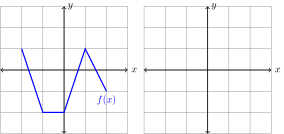
\includegraphics[width=0.65\columnwidth]{figures/0-3-fig2.pdf}
        \end{center}
        \caption{Function transformation for Activity \ref{A:0.3.1}} \label{F:0.3.Act1}
    \end{figure}
\end{activity}
\begin{smallhint}
    \ba
        \item Think of the ``$-$'' in front of $f(x)$ as a $-1$.  What is the difference
            between multiplying by $-1$ and adding $-1$?
        \item Think about the order of mathematical operations.
    \ea
\end{smallhint}
\begin{bighint}
    \ba
        \item $g(x)$ should be a vertical stretch and $h(x)$ should be a vertical shift.
        \item A very methodical way to approach this problem would be to choose several
            particular $x$ values and follow the order of operations to determine the
            output for $k$.
    \ea
\end{bighint}
\begin{activitySolution}
    \ba
        \item The function $g(x)$ should change the sign on all of the $y$ values of $f$.
            The function $h(x)$ will shift all of the $y$ values of $f$ down 1 unit.
        \item The order in which you do the transformations does matter.  In this problem
            the order of operations should be to change the sign on the $y$ value and then
            to shift 1 unit down.
    \ea
    \begin{center}
        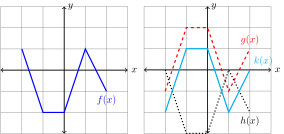
\includegraphics[width=0.65\columnwidth]{figures/0-3-fig2soln.pdf}
    \end{center}
\end{activitySolution}

\aftera

\newpage
\begin{activity}\label{A:0.3.2}
    \ba
        \item Let $f(x) = x^2$ and $g(x) = x+8$.  Find the following:
            \[ f(g(3)) = \underline{\hspace{1in}}, \quad g(f(3)) =
                \underline{\hspace{1in}}, \quad f(g(x)) = \underline{\hspace{1in}},\]
            \[ g(f(x)) = \underline{\hspace{1in}}, \quad f(x)g(x) = \underline{\hspace{1in}}
                \]
        \item Now let $f(x)$ and $g(x)$ be defined as in the table below.  Use the data in
            the table to find the following compositions.
            \begin{center}
                \begin{tabular}{|c||c|c|c|c|c|c|c|}
                    \hline
                    $x$ & $-3$ & $-2$ & $-1$ & $0$ & $1$ & $2$ & $3$ \\ \hline \hline
                    $f(x)$ & 3 & 1 & $-1$ & $-3$ & $-1$ & 1 & 3 \\ \hline
                    $g(x)$ & $-2$ & $-1$ & 0 & 1 & 0 & 1 & 2 \\ \hline
                \end{tabular}
            \end{center}
            \[ 
                f(-3) = \underline{\hspace{1in}}, \quad
                g(3) = \underline{\hspace{1in}}, \]
            \[  f(g(-3)) = \underline{\hspace{1in}}, \quad
                f(g(f(-3))) = \underline{\hspace{1in}} \quad
                \]
        \item Now let $f(x)$ and $g(x)$ be defined as in the plots below.  Use the plots
            to find the following compositions.
%             \begin{figure}
%                 \begin{center}
%                     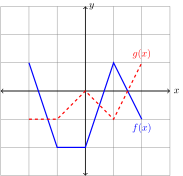
\includegraphics[width=0.6\columnwidth]{figures/0-3-fig3.pdf}
%                 \end{center}
%                 \caption{The functions $f(x)$ and $g(x)$ for Activity \ref{A:0.3.2}.}
%                 \label{f:A:0.3.2}
%             \end{figure}

            \begin{minipage}{0.5\columnwidth}
                \begin{center}
                    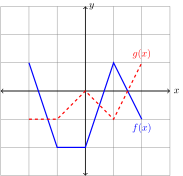
\includegraphics[width=0.9\columnwidth]{figures/0-3-fig3.pdf}
                \end{center}
            \end{minipage}
            \begin{minipage}{0.4\columnwidth}
                \begin{flalign*}
                    f(1) &= \underline{\hspace{1in}} \\
                    g(2) &= \underline{\hspace{1in}} \\
                    g(f(1)) &= \underline{\hspace{1in}} \\
                    f(g(1)) &= \underline{\hspace{1in}} \\
                    g(f(f(0))) &= \underline{\hspace{1in}}
                \end{flalign*}
                
            \end{minipage}
    \ea

\end{activity}
\begin{smallhint}
    \ba
        \item Start from the inside and work your way out.  The first two answers will be
            numbers and the next three will be functions.
        \item The numbers on the inside of the table are the $y$ values for the functions
            $f$ and $g$.  
        \item You're looking for the $y$ values that come out of these functions.
    \ea
\end{smallhint}
\begin{bighint}
    \ba
        \item On the function compositions, first evaluate the expression inside the
            parenthesis.  Then evaluate the outside.
        \item For an expression such as $f(g(-3))$, first evaluate $g(-3)$ and then
            substitute the answer into $f$.
        \item The same hints apply to the graphical version of the problem.
    \ea
\end{bighint}
\begin{activitySolution}
    \ba
        \item For $f(x) = x^2$ and $g(x) = x+8$
            \begin{flalign*}
                f(g(3)) &= f(11) = 121 \\
                g(f(3)) &= g(9) = 17 \\
                f(g(x)) &= f(x+8) = (x+8)^2 \\
                g(f(x)) &= g(x^2) = x^2 + 8 \\
                f(x)g(x) &=(x^2)(x+8) = x^3 + 8x^2 
            \end{flalign*}
        \item
            \begin{flalign*}
                f(-3) &= 3 \\
                g(3) &= 2 \\
                f(g(-3)) &= f(-2) = 1 \\
                f(g(f(-3))) &= f(g(3)) = f(2) = 1
            \end{flalign*}
        \item 
            \begin{flalign*}
                f(1) &= 1 \\
                g(2) &= 1 \\
                g(f(1)) &= g(1) = -1 \\
                f(g(1)) &= f(-1) = -2 \\
                g(f(f(0))) &= g(f(-2)) = g(1) = 1
            \end{flalign*}
    \ea
\end{activitySolution}


\aftera

\newpage
\subsection*{Voting Questions}
\renewcommand{\labelenumi}{\thesection.\arabic{enumi}}
\begin{enumerate}
        \input{clicker/SVC.01.03.010.tex}
        \teacher{\input{clicker/SVC.01.03.010C.tex}}
        \input{clicker/SVC.01.03.020.tex}
        \teacher{\input{clicker/SVC.01.03.020C.tex}}
        \input{clicker/SVC.01.03.030.tex}
        \teacher{\input{clicker/SVC.01.03.030C.tex}}
        \input{clicker/SVC.01.03.040.tex}
        \teacher{\input{clicker/SVC.01.03.040C.tex}}
        \input{clicker/SVC.01.03.050.tex}
        \teacher{\input{clicker/SVC.01.03.050C.tex}}
        \input{clicker/SVC.01.03.051.tex}
        \teacher{\input{clicker/SVC.01.03.051C.tex}}
        \input{clicker/SVC.01.03.052.tex}
        \teacher{\input{clicker/SVC.01.03.052C.tex}}
        \input{clicker/SVC.01.03.053.tex}
        \teacher{\input{clicker/SVC.01.03.053C.tex}}
        \input{clicker/SVC.01.03.054.tex}
        \teacher{\input{clicker/SVC.01.03.054C.tex}}
        \input{clicker/SVC.01.03.055.tex}
        \teacher{\input{clicker/SVC.01.03.055C.tex}}
        \input{clicker/SVC.01.03.056.tex}
        \teacher{\input{clicker/SVC.01.03.056C.tex}}
        \input{clicker/SVC.01.03.060.tex}
        \teacher{\input{clicker/SVC.01.03.060C.tex}}
        \input{clicker/SVC.01.03.065.tex}
        \teacher{\input{clicker/SVC.01.03.065C.tex}}
        \input{clicker/SVC.01.03.070.tex}
        \teacher{\input{clicker/SVC.01.03.070C.tex}}
        \input{clicker/SVC.01.03.071.tex}
        \teacher{\input{clicker/SVC.01.03.071C.tex}}
        \input{clicker/SVC.01.03.072.tex}
        \teacher{\input{clicker/SVC.01.03.072C.tex}}
        \input{clicker/SVC.01.03.075.tex}
        \teacher{\input{clicker/SVC.01.03.075C.tex}}
        \input{clicker/SVC.01.03.076.tex}
        \teacher{\input{clicker/SVC.01.03.076C.tex}}
        \input{clicker/SVC.01.03.080.tex}
        \teacher{\input{clicker/SVC.01.03.080C.tex}}
        \input{clicker/SVC.01.03.090.tex}
        \teacher{\input{clicker/SVC.01.03.090C.tex}}
        \input{clicker/SVC.01.03.100.tex}
        \teacher{\input{clicker/SVC.01.03.100C.tex}}
        \input{clicker/SVC.01.03.102.tex}
        \teacher{\input{clicker/SVC.01.03.102C.tex}}
        \input{clicker/SVC.01.03.110.tex}
        \teacher{\input{clicker/SVC.01.03.110C.tex}}
        \input{clicker/SVC.01.03.120.tex}
        \teacher{\input{clicker/SVC.01.03.120C.tex}}
        \input{clicker/SVC.01.03.130.tex}
        \teacher{\input{clicker/SVC.01.03.130C.tex}}
        \input{clicker/SVC.01.03.140.tex}
        \teacher{\input{clicker/SVC.01.03.140C.tex}}
        \input{clicker/SVC.01.03.150.tex}
        \teacher{\input{clicker/SVC.01.03.150C.tex}}
\end{enumerate}
\renewcommand{\labelenumi}{\arabic{enumi}}

\newpage

\section{Logarithmic Functions} \label{S:0.4.Logarithms}

\begin{pa} \label{PA:0.4}
	Carbon-14 ($^{14}$C) is a radioactive isotope of carbon that occurs naturally in the Earth's atmosphere.  During photosynthesis, plants take in $^{14}$C along with other carbon 	isotopes, and the levels of  $^{14}$C in living plants are roughly the same as atmospheric levels.  Once a plant dies, it no longer takes in any additional  $^{14}$C.  Since  $^{14}$C in the dead plant decays at a predictable rate (the half-life of $^{14}$C is approximately 5,730 years), we can measure  $^{14}$C levels in dead plant matter to get an estimate on how long ago the plant 	died.
	Suppose that a plant has 0.02 milligrams of $^{14}$C when it dies.
\ba
	\item Write a function that represents the amount of $^{14}$C remaining in the plant after $t$ years.
	\item Complete the table for the amount of $^{14}$C remaining $t$ years after the death of the plant.
        \begin{center}
            \begin{tabular}[h!]{| l |c|c|c|c|c|c|c|c|}
                \hline
                t & 0 & 1 & 5 & 10 & 100 & 1000 & 2000 & 5730 \\ \hline
                $^{14}$C Level & 0.02 & & & & & & & \\ \hline
            \end{tabular}
        \end{center}
	\item Suppose our plant died sometime in the past.  If we find that there are 0.014 milligrams of $^{14}$C present in the plant now, estimate the age of the plant to within 50 years.
        \ea
\end{pa} \afterpa

\newpage
\begin{activity}\label{A:0.4.1}
    Use the definition of a logarithm along with the properties of logarithms to answer
    the following.
    \ba
\item Write the exponential expression $8^{1/3} = 2$ as a logarithmic expression.
\item Write the logarithmic expression $\log_2 \frac{1}{32} = -5$ as an exponential
    expression.
\item What value of $x$ solves the equation $\log_2 x = 3$?
\item What value of $x$ solves the equation $\log_2 4 = x$?
\item Use the laws of logarithms to rewrite the expression $\log \left( x^3 y^5 \right)$
    in a form with no logarithms of products, quotients, or powers.
\item Use the laws of logarithms to rewrite the expression $\log \left( \frac{x^{15}
    y^{20}}{z^4} \right)$
    in a form with no logarithms of products, quotients, or powers.
\item Rewrite the expression $\ln(8) + 5 \ln(x) + 15 \ln(x^2+8)$ as a single logarithm.
    \ea


\end{activity}
\begin{smallhint}
    Use the properties of logarithms.
\end{smallhint}
\begin{bighint}
    Use the properties of logarithms.
\end{bighint}
\begin{activitySolution}
    \ba
\item $8^{1/3} = 2$ is equivalent to $\log_8 2 = \frac{1}{3}$.
\item $\log_2 \frac{1}{32} = -5$ is equivalent to $2^{-5} = \frac{1}{32}$.
\item $\log_2 x = 3$ is equivalent to $x = 2^3 = 8$.
\item $\log_2 4 = x$ is equivalent to $2^x = 4$ and we see that $x=2$ since $2^2 = 4$.
\item Using the product and power properties
    \[ \log\left( x^3 y^5 \right) = 3\log(x) + 5\log(y). \]
\item Using the product, power, and quotient properties
    \[ \log\left( \frac{x^{15} y^{20}}{z^4} \right) = 15\log(x) + 20\log(y) - 4\log(z). \]
\item Using the power and product properties
    \[ \ln(8) + 5 \ln(x) + 15\ln(x^2+8) = \ln\left( 8 x^5 \left( x^2 + 8 \right)^{15}
        \right) \]
    \ea
\end{activitySolution}

\aftera

\newpage
\begin{activity}\label{A:0.4.2}
    Solve each of the following equations for $t$, and verify your answers using a calculator.
	\ba
		\item $\ln t=4$
		\item $\ln(t+3)=4$
		\item $\ln(t+3)=\ln4$
		\item $\ln(t+3)+\ln(t)=\ln4$
		\item $e^{t}=4$
		\item $e^{t+3}=4$
		\item $2e^{t+3}=4$
		\item $2e^{3t+2}=3e^{t-1}$
	\ea

\end{activity}
\begin{smallhint}
    
\end{smallhint}
\begin{bighint}
    
\end{bighint}
\begin{activitySolution}
    \ba
        \item $t = e^4$
        \item $t+3 = e^4$ so $t = e^4 - 3$
        \item $t+3 = 4$ so $t=1$
        \item Using the product property for logarithms, $\ln(t(t+3)) = \ln(4)$ so $t^2 +
            3t = 4$.  This is quadratic so we rearrange to get $t^2 + 3t - 4 = 0$ which
            factors to $(t+4)(t-1) = 0$ so the solutions are $t=1$ and $t=-4$.
            Substituting back to the original equation we see that $\ln(-4+3)$ and
            $\ln(-4)$ do not exist so the only solution is $t=1$.
        \item $t=\ln(4)$
        \item $t= \ln(4) = 3$
        \item $t+3 = \ln(2)$ so $t = \ln(2) = 3$
        \item For the final problem we first divide by $2$ and take the natural logarithm
            of both sides.
            \[ e^{3t+1} = \frac{3}{2} e^{t-1} \implies 3t+1 = \ln(3/2) + t-1. \]
            Therefore, $2t = \ln(3/2) - 2$ so $t=\frac{1}{2} \left( \ln(3/2) - 2 \right)$.
    \ea
\end{activitySolution}
\aftera

\newpage
\begin{activity}\label{A:0.4.3}
    Consider the following equation:
	\[
		7^{x} = 24
	\]

	\ba
		\item How many solutions should we expect to find for this equation?
		\item Solve the equation using the log base 7.
		\item Solve the equation using the log base 10.
		\item Solve the equation using the natural log.
		\item Most calculators have buttons for $\log_{10}$ and $\ln$, but none have a button for $\log_{7}$. Use your previous answers to write a formula for $\log_{7}x$ in terms of 					$\log x$ or $\ln x$.
	\ea

\end{activity}\aftera

\newpage
\begin{activity}\label{A:0.4.4}
\ba
\item In the presence of sufficient resources the population of a colony of bacteria exhibits exponential growth, doubling once every three hours. What is the corresponding continuous (percentage) growth rate?
\item A hot bowl of soup is served at a dinner party.  It starts to cool according to
    Newton's Law of Cooling so its temperature, $T$ (measured in degrees Fahrenheit) after
    $t$ minutes is given by
    \[ T(t) = 65 + 186 e^{-0.06t}. \]
    How long will it take from the time the food is served until the temperature is
    $120^\circ$F?
\item The velocity (in ft/sec) of a sky diver $t$ seconds after jumping is given by 
    \[ v(t) = 80\left( 1-e^{-0.2t} \right). \]
    After how many seconds is the velocity 75 ft/sec?
\ea
\end{activity}
\begin{smallhint}
    Use the properties of logarithms.
\end{smallhint}
\begin{bighint}
    Use the properties of logarithms.
\end{bighint}
\begin{activitySolution}
    \ba
        \item If the population doubles every three hours then the exponential function
            describing the growth is $P(t) = P_0 2^{t/3}$.  We want to find the continuous
            growth rate so we want to write the function as $P(t) = P_0 e^{kt}$.
            Therefore we need to solve the equation $2^{t/3} = e^{kt}$ for $k$.  Taking
            the natural logarithm of both sides gives
            $\ln \left( 2^{t/3} \right) = kt$, and using the rules of exponents we see
            that $\frac{t}{3} \ln(2) = kt$.  Subtracting $kt$ from both sides and
            factoring the $t$ gives $t\left( \frac{\ln(2)}{3} - k \right) = 0$ so we
            immediately see that $k = \ln(2)/3$.
        \item We need to solve the equation $65+186e^{-0.06t} = 120$.  Subtracting 65 and
            dividing by 186 gives $e^{-0.06t} = \frac{55}{186}$.  Taking the natural
            logarithm of both sides and then dividing by -0.06 gives $t =
            -\frac{1}{0.06} \ln \left( \frac{55}{186} \right)$.
        \item We need to solve the equation $80\left( 1-e^{-0.2t} \right) = 75$.  Dividing
            by 80 gives $1-e^{-0.2t} = \frac{15}{16}$.  Hence, $e^{-0.2t} =
            \frac{1}{16}$ and taking the natural logarithm of both sides gives $-0.2t =
            \ln(1/16)$.  Therefore, $t = -\frac{1}{0.2} \ln\left( \frac{1}{16} \right)$.
    \ea
\end{activitySolution}

\aftera

\newpage
\subsection*{Voting Questions}
\renewcommand{\labelenumi}{\thesection.\arabic{enumi}}
\begin{enumerate}
        \input{clicker/SVC.01.04.005.tex}
        \teacher{\input{clicker/SVC.01.04.005C.tex}}
        \input{clicker/SVC.01.04.010.tex}
        \teacher{\input{clicker/SVC.01.04.010C.tex}}
        \input{clicker/SVC.01.04.020.tex}
        \teacher{\input{clicker/SVC.01.04.020C.tex}}
        \input{clicker/SVC.01.04.024.tex}
        \teacher{\input{clicker/SVC.01.04.024C.tex}}
        \input{clicker/SVC.01.04.025.tex}
        \teacher{\input{clicker/SVC.01.04.025C.tex}}
        \input{clicker/SVC.01.04.026.tex}
        \teacher{\input{clicker/SVC.01.04.026C.tex}}
        \input{clicker/SVC.01.04.027.tex}
        \teacher{\input{clicker/SVC.01.04.027C.tex}}
        \input{clicker/SVC.01.04.030.tex}
        \teacher{\input{clicker/SVC.01.04.030C.tex}}
        \input{clicker/SVC.01.04.040.tex}
        \teacher{\input{clicker/SVC.01.04.040C.tex}}
        \input{clicker/SVC.01.04.050.tex}
        \teacher{\input{clicker/SVC.01.04.050C.tex}}
        \input{clicker/SVC.01.04.051.tex}
        \teacher{\input{clicker/SVC.01.04.051C.tex}}
        \input{clicker/SVC.01.04.052.tex}
        \teacher{\input{clicker/SVC.01.04.052C.tex}}
        \input{clicker/SVC.01.04.053.tex}
        \teacher{\input{clicker/SVC.01.04.053C.tex}}
        \input{clicker/SVC.01.04.054.tex}
        \teacher{\input{clicker/SVC.01.04.054C.tex}}
        \input{clicker/SVC.01.04.055.tex}
        \teacher{\input{clicker/SVC.01.04.055C.tex}}
        \input{clicker/SVC.01.04.056.tex}
        \teacher{\input{clicker/SVC.01.04.056C.tex}}
        \input{clicker/SVC.01.04.057.tex}
        \teacher{\input{clicker/SVC.01.04.057C.tex}}
        \input{clicker/SVC.01.04.060.tex}
        \teacher{\input{clicker/SVC.01.04.060C.tex}}
        \input{clicker/SVC.01.04.070.tex}
        \teacher{\input{clicker/SVC.01.04.070C.tex}}
        \input{clicker/SVC.01.04.080.tex}
        \teacher{\input{clicker/SVC.01.04.080C.tex}}
        \input{clicker/SVC.01.04.085.tex}
        \teacher{\input{clicker/SVC.01.04.085C.tex}}
        \input{clicker/SVC.01.04.090.tex}
        \teacher{\input{clicker/SVC.01.04.090C.tex}}
        \input{clicker/SVC.01.04.095.tex}
        \teacher{\input{clicker/SVC.01.04.095C.tex}}
        \input{clicker/SVC.01.04.100.tex}
        \teacher{\input{clicker/SVC.01.04.100C.tex}}
        \input{clicker/SVC.01.04.110.tex}
        \teacher{\input{clicker/SVC.01.04.110C.tex}}
\end{enumerate}
\renewcommand{\labelenumi}{\arabic{enumi}}

\newpage

\section{Trigonometric Functions} \label{S.0.5.TrigFunctions}

\begin{pa} \label{PA:0.5}
A tall water tower is swaying back and forth in the wind.  Using an ultrasonic ranging
device, we measure the distance from our device to the tower (in centimeters) every two
seconds with these measurements recorded below.  

\medskip

\begin{tabular}{| c | c | c | c | c | c | c | c | c | c | c | c |}
\hline
Time (sec) & 0 & 2 & 4 & 6 & 8 & 10 & 12 & 14 & 16 & 18 & 20 \\
\hline
Distance (cm) & 30.9 & 23.1 & 14.7 & 12.3 & 17.7 & 26.7 & 32.3 & 30.1 & 21.8 & 13.9 & 12.6 \\
\hline
\end{tabular}

% \begin{enumerate}
\ba
\item Use the coordinate plane below to create a graph of these data points.
    \begin{center}
        \begin{tikzpicture}
            \begin{axis}[axis lines=center, xmin=-0.5, xmax=20, ymin=0, ymax=40,
                xtick={2,4,6,8,10,12,14,16,18,20}, ytick={5,10,15,20,25,30,35,40}, grid,
            xlabel={Time (sec)}, ylabel={Distance (cm)}]
                \addplot[smooth] {0*x};
            \end{axis}
        \end{tikzpicture}
    \end{center}
\item What is the water tower's maximum distance away from the device? % 32.3 cm
\item What is the smallest distance measured from the tower to the device? % 12.3 cm
\item If the water tower was sitting still and no wind was blowing, what would be the distance from the tower to the device?  We call this the tower's equilibrium position.% About 22.3 cm
\item What is the maximum distance that the tower moves away from its equilibrium position?  We call this the amplitude of the oscillations.  % About 10 centimeters
\item How much time does it take the water tower to sway back and forth in a complete cycle?  We call this the period of oscillation.  % About 14 seconds
% \end{enumerate}



\ea
\end{pa} \afterpa

\newpage
\begin{activity}\label{A:0.5.1}
    Figure \ref{fig:0.5.A1} gives us the voltage produced by an electrical circuit as a function of time.
    \begin{figure}[ht!]
    \begin{center}
%         \begin{tikzpicture}
%             \begin{axis}[axis lines=center, xmin=0, xmax=0.05, ymin=-15, ymax=55, grid,
%                     domain=0:0.05, xlabel={time (sec)}, ylabel={volts},
%                     xtick={0.005,0.01,0.015,0.02,0.025,0.03,0.035,0.04,0.045,0.05},
%                     xticklabels={0.005,0.01,0.015,0.02,0.025,0.03,0.035,0.04,0.045,0.05},
%                 ytick={-10,10,20,30,40,50}, xscale=2]
%                 \addplot[smooth, very thick, blue, samples=100]
%                 {30*sin(deg(2*pi/0.017*(x-0.008)))+20};
%             \end{axis}
%         \end{tikzpicture}
        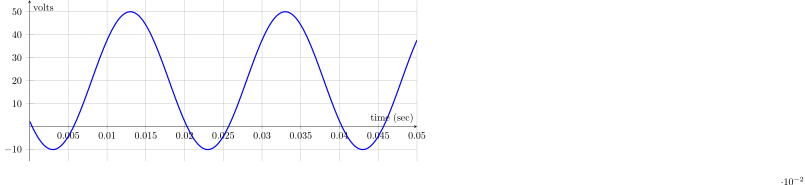
\includegraphics[trim=0cm 0cm 12cm 0cm, clip, width=0.9\columnwidth]{figures/0-5-fig9.pdf}
    \end{center}
    \caption{Voltage as a function of time.}
    \label{fig:0.5.A1}
\end{figure}
% \resizebox{5in}{!}{\includegraphics{0-5-TrigonometricFunctions5.jpg}}


\ba
\item What is the amplitude of the oscillations?  % 30 volts
\item What is the period of the oscillations? % about 0.017 seconds
\item What is the average value of the voltage?  % 20 volts
\item What is the shift along the $t$ axis, $t_0$?  % about 0.008 seconds
\item What is a formula for this function?  %  V(t) = 30 \sin( 2\pi / 0.017 ( t - 0.008) ) + 20
\ea

\end{activity}
\begin{smallhint}
    \ba
        \item measure the amplitude at half the maximum minus the minimum.
        \item measure the period from peak to peak or from trough to trough.
        \item the average value comes from the $y$ values.
        \item find the middle of the voltage values.
        \item be sure to get the shift correct.  
        \item There are infinitely many answers to this
            problem!
    \ea
\end{smallhint}
\begin{bighint}
    \ba
        \item measure the amplitude at half the maximum minus the minimum.
        \item measure the period from peak to peak or from trough to trough.
        \item the average value comes from the $y$ values.
        \item find the middle of the voltage values.
        \item be sure to get the shift correct.  
        \item There are infinitely many answers to this
            problem!
    \ea
\end{bighint}
\begin{activitySolution}
   \ba
    \item The amplitude is $A = \frac{1}{2}(50-(-10)) = 30$.
    \item The period is the distance from peak to peak.  In this case there is a peak at
        approximately $t=0.0125$ seconds and $t = 0.0325$ seconds.  Hence, the period is
        $0.02$ seconds.
    \item The average value of the voltage is 20.
    \item The simplest shift is probably to the first peak at $t = 0.0125$ seconds.
    \item $V(t) = 30 \cos\left( \frac{2\pi}{0.02} \left( t - 0.0125 \right) \right) + 20$.
   \ea
\end{activitySolution}

\aftera

\newpage
\begin{activity}\label{A:0.5.2}
Suppose the following sinusoidal function models the water level on a pier in the ocean as
it changes due to the tides during a certain day.
\[ w(t) = 4.3 \sin \left( 0.51 t + 0.82 \right) + 10.6 \]
\ba
\item Using the formula above, make a table showing the water level every two hours for a 24 hour period starting at midnight.
    \begin{center}
        \begin{tabular}[h!]{|c||c|c|c|c|c|c|c|c|c|c|c|c|c|}
            \hline
            time (hours) & 0 & 2 & 4 & 6 & 8 & 10 & 12 & 14 & 16 & 18 & 20 & 22 & 24 \\
            \hline
            water level (ft) & & & & & & & & & & & & & \\ \hline
        \end{tabular}
    \end{center}
\item Sketch a graph of this function using the data from your table in part (a).
    \begin{center}
%         \begin{tikzpicture}
%             \begin{axis}[ymin=0, ymax=20, xmin=0, xmax=24, domain=0:24,
%                 grid, xtick={2,4,6,8,10,12,14,16,18,20,22,24},
%             ytick={0,2,4,6,8,10,12,14,16,18,20}, xlabel={time (hours)}, ylabel={water level
%             (ft)}, xscale=1.25]
%                 \addplot[smooth] {0*x};
%             \end{axis}
%         \end{tikzpicture}
        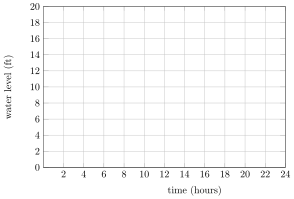
\includegraphics[width=0.6\columnwidth]{figures/0-5-fig10.pdf}
    \end{center}
\item What is the period of oscillation of this function? % Period $ = 2 \pi / B \approx  12.3$ hours.
\item What time is high tide?  % The sine function reaches a peak when its input is $\pi/2$.  So $0.51 t + 0.82 = \pi/2$ and $t = 1.47$ hours, or about 1:30 am.

\ea
\end{activity}\aftera

\newpage

\subsection*{Voting Questions}
\renewcommand{\labelenumi}{\thesection.\arabic{enumi}}
\begin{enumerate}
        \input{clicker/SVC.01.05.005.tex}
        \teacher{\input{clicker/SVC.01.05.005C.tex}}
        \input{clicker/SVC.01.05.010.tex}
        \teacher{\input{clicker/SVC.01.05.010C.tex}}
        \input{clicker/SVC.01.05.015.tex}
        \teacher{\input{clicker/SVC.01.05.015C.tex}}
        \input{clicker/SVC.01.05.020.tex}
        \teacher{\input{clicker/SVC.01.05.020C.tex}}
        \input{clicker/SVC.01.05.030.tex}
        \teacher{\input{clicker/SVC.01.05.030C.tex}}
        \input{clicker/SVC.01.05.040.tex}
        \teacher{\input{clicker/SVC.01.05.040C.tex}}
        \input{clicker/SVC.01.05.050.tex}
        \teacher{\input{clicker/SVC.01.05.050C.tex}}
        \input{clicker/SVC.01.05.055.tex}
        \teacher{\input{clicker/SVC.01.05.055C.tex}}
        \input{clicker/SVC.01.05.060.tex}
        \teacher{\input{clicker/SVC.01.05.060C.tex}}
        \input{clicker/SVC.01.05.070.tex}
        \teacher{\input{clicker/SVC.01.05.070C.tex}}
        \input{clicker/SVC.01.05.075.tex}
        \teacher{\input{clicker/SVC.01.05.075C.tex}}
        \input{clicker/SVC.01.05.080.tex}
        \teacher{\input{clicker/SVC.01.05.080C.tex}}
        \input{clicker/SVC.01.05.085.tex}
        \teacher{\input{clicker/SVC.01.05.085C.tex}}
        \input{clicker/SVC.01.05.090.tex}
        \teacher{\input{clicker/SVC.01.05.090C.tex}}
        \input{clicker/SVC.01.05.095.tex}
        \teacher{\input{clicker/SVC.01.05.095C.tex}}
        \input{clicker/SVC.01.05.100.tex}
        \teacher{\input{clicker/SVC.01.05.100C.tex}}
\end{enumerate}
\renewcommand{\labelenumi}{\arabic{enumi}}

\newpage

\section{Powers, Polynomials, and Rational Functions} \label{S.0.6.PowersPolysRationals}

\begin{pa} \label{PA:0.6}
    
Figure \ref{fig:0.6.PA} shows the graphs of two different functions.  Suppose that you were to graph a line anywhere along each of the two graphs.

\begin{enumerate}
	\item Is it possible to draw a line that does not intersect the graph of $f$? $g$?
	\item Is it possible to draw a line that intersects the graph of $f$ an even number of times?
	\item Is it possible to draw a line that intersects the graph of $g$ an odd number of times?
	\item What is the fewest number of intersections that your line could have with the graph of $f$? with $g$?
	\item What is the largest number of intersections that your line could have with the graph of $f$? with $g$?
	\item How many times does the graph of $f$ change directions? How many times does the graph of $g$ change directions?
\end{enumerate}

\begin{figure}[ht!]

	\begin{center}
		\begin{tikzpicture}[scale=0.75]
			[line cap=round,line join=round,>=triangle 45,x=1.0cm,y=1.0cm] 
			\draw[<->,color=black] (-4.418087504107611,0.0) -- (5.504275777242757,0.0); \foreach \x in {-4.0,-3.0,-2.0,-1.0,1.0,2.0,3.0,4.0,5.0} 
			\draw[shift={(\x,0)},color=black] (0pt,2pt) -- (0pt,-2pt); 
			\draw[<->] (0.0,-2.486833997057605) -- (0.0,5.09438316608086); \foreach \y in {-2.0,-1.0,1.0,2.0,3.0,4.0,5.0} 
			\draw[shift={(0,\y)},color=black] (2pt,0pt) -- (-2pt,0pt); 
			\clip(-4.418087504107611,-2.486833997057605) rectangle (5.504275777242757,5.09438316608086); 
			\draw[color=blue, very thick,smooth,samples=100,domain=-3.3:4.5]
			plot(\x,{((\x)-1.1)^(2.0)*((\x)-3.6)*((\x)+1.5)*((\x)-4.2)*((\x)+2.2)*((\x)+3.1)/100.0});
			\begin{scriptsize}
				\draw[color=black] (5,4.671245463952202) node {$f(x)$};
			\end{scriptsize}
		\end{tikzpicture}
		\begin{tikzpicture}[scale=0.75]
			[line cap=round,line join=round,>=triangle 45,x=1.0cm,y=1.0cm] 
			\draw[<->,color=black] (-4.418087504107611,0.0) -- (5.504275777242757,0.0); \foreach \x in {-4.0,-3.0,-2.0,-1.0,1.0,2.0,3.0,4.0,5.0} 
			\draw[shift={(\x,0)},color=black] (0pt,2pt) -- (0pt,-2pt); 
			\draw[<->,color=black] (0.0,-2.486833997057605) -- (0.0,5.09438316608086); \foreach \y in {-2.0,-1.0,1.0,2.0,3.0,4.0,5.0} 
			\draw[shift={(0,\y)},color=black] (2pt,0pt) -- (-2pt,0pt); 
			\clip(-4.418087504107611,-2.486833997057605) rectangle (5.504275777242757,5.09438316608086); 
			\draw[color=blue, very thick,smooth,samples=100,domain=-4:5]
			plot(\x,{((\x)-1.1)*((\x)-3.6)*((\x)+1.5)*((\x)-4.2)*((\x)+2.2)*((\x)+3.1)/100.0});
			\begin{scriptsize}
				\draw[color=black] (5.1,4.671245463952202) node {$g(x)$};
			\end{scriptsize}
		\end{tikzpicture} 
	\end{center}      
\caption{$f(x)$ and $g(x)$ for the preview activity.}
\label{fig:0.6.PA}
\end{figure}


\end{pa} \afterpa

\newpage
\begin{activity}\label{A:0.6.1}
Power functions and exponential functions appear somewhat similar in their formulas, but behave differently in many ways.  
\ba
	\item Compare the functions $f(x)=x^2$ and $g(x)=2^x$ by graphing both functions in several viewing windows.  Find the points of intersection of the graphs.  Which function grows more rapidly when $x$ is large?
    \item Compare the functions $f(x)=x^{10}$ and $g(x)=2^x$ by graphing both functions in several viewing windows.  Find the points of intersection of the graphs.  Which function grows more rapidly when $x$ is large?
	\item Make a conjecture: As $x\to\infty$, which dominates, $x^n$ or $a^x$ for $a>1$?
% 	\item Suppose you are offered a job that lasts one month.  You have the option of being paid in one of two ways: (1) One million dollars at the end of the month; or (2) One cent on the first day of the month, two cents on the second day, four cents on the third day, and, in general, $2^{n-1}$ cents on the $n^{th}$ day.  Which option should you choose?
% 	\item How much different (shorter or longer) would the work period need to be for your answer to the previous question change?
        \ea

\end{activity}
\begin{smallhint}
You may need to use a graphing tool for this activity.
\end{smallhint}
\begin{bighint}
You may need to use a graphing tool for this activity. To see the full behavior of the
functions you will need to use the zoom and pan tools on your graphing technology.
\end{bighint}
\begin{activitySolution}
   \ba
        \item The functions $f(x) = x^2$ and $g(x) = 2^x$ intersect at three points:
            $(-0.77,0.59)$, $(2,4)$, and $(4,16)$.  After the point $(4,16)$ the
            exponential function $g(x) = 2^x$ grows more rapidly.
        \item The functions $f(x) = x^{10}$ and $g(x) = 2^x$ intersect at three points:
            $(-0.94, 0.52)$, $(1.08, 2.11)$, and another point near $x \approx 60$.  The
            $y$ values on both functions at the third point are very very large, but at
            this point the function $g(x) = 2^x$ dominates the power function $f(x) =
            x^{10}$.
        \item For $a>1$ the exponential function will always dominate the power function.
        \item 
   \ea
\end{activitySolution}

\aftera

\newpage
\begin{activity}\label{A:0.6.2}
	For each of the following graphs, find a possible formula for the polynomial of lowest degree that fits the graph.
    \def\scl{0.7}
				\begin{center}
%                     \begin{tikzpicture}[scale=\scl]
%                         \begin{axis}[axis lines=center, xmin=-4, xmax=2, ymin=-5, ymax=2,
%                             title={Plot (a)}]
%                             \addplot[very thick, blue, smooth,samples=100,domain=-4.0:2.0] {((x)-1.0)*((x)+3.0)};
%                         \end{axis}
%                     \end{tikzpicture}
%                     \begin{tikzpicture}[scale=\scl]
%                         \begin{axis}[axis lines=center, xmin=-3, xmax=3.5, ymin=-8.5, ymax=6,
%                             title={Plot (b)}, ytick={-8,-6,-4,-2,2,4,6}]
%                             \addplot[very thick, blue, smooth,samples=100,domain=-3:3.5] {0-((x)+2.0)*((x)-3.0)*((x)-1.0)};
%                         \end{axis}
%                     \end{tikzpicture}
%                     \begin{tikzpicture}[scale=\scl]
%                         \begin{axis}[axis lines=center, xmin=-2, xmax=3, ymin=-3, ymax=2,
%                             title={Plot (c)}]
%                             \addplot[very thick, blue, smooth,samples=100,domain=-2:3] {((x)+1.0)*((x)-2.0)*((x)-1.0)*((x)-1.0)};
%                         \end{axis}
%                     \end{tikzpicture}
% % 					\begin{tikzpicture}[line cap=round,line join=round,>=triangle 45, x=1.0cm, y=0.86cm] 
% % 						\draw[->,color=black] (-4.0,0.0) -- (2.0,0.0);
% % 						\foreach \x in {-4,-3,-2,-1,1}
% % 						\draw[shift={(\x,0)},color=black] (0pt,2pt) -- (0pt,-2pt) node[below] {\footnotesize $\x$};
% % 						\draw[->,color=black] (0.0,-5.0) -- (0.0,2.0);
% % 						\foreach \y in {-5,-4,-3,-2,-1,1}
% % 						\draw[shift={(0,\y)},color=black] (2pt,0pt) -- (-2pt,0pt) node[left] {\footnotesize $\y$};
% % 						\draw[color=black] (0pt,-10pt) node[right] {\footnotesize $0$};
% % 						\clip(-4.0,-5.0) rectangle (2.0,2.0);
% % 						\draw[very thick, blue, smooth,samples=100,domain=-4.0:2.0] plot(\x,{((\x)-1.0)*((\x)+3.0)});
% % 					\end{tikzpicture}   
% % 					\begin{tikzpicture}[line cap=round,line join=round,>=triangle 45, x=0.86cm, y=0.33cm] 
% % 						\draw[<->,color=black] (-3.5,0.0) -- (3.5,0.0); 
% % 						\foreach \x in {-3,-2,-1,1,2,3} 
% % 						\draw[shift={(\x,0)},color=black] (0pt,2pt) -- (0pt,-2pt) node[below] {\footnotesize $\x$}; 
% % 						\draw[->,color=black] (0.0,-10) -- (0.0,8); 
% % 						\foreach \y in {-8,-6,-4,-2,2,4,6}
% % 						\draw[shift={(0,\y)},color=black] (2pt,0pt) -- (-2pt,0pt) node[left] {\footnotesize $\y$}; 
% % 						\draw[color=black] (0pt,-10pt) node[right] {\footnotesize $0$}; 
% % 						\clip(-3.5,-10) rectangle (3.5,8); 
% % 						\draw[very thick, blue, smooth,samples=100,domain=-3.5:3.5] plot(\x,{0-((\x)+2.0)*((\x)-3.0)*((\x)-1.0)});
% % 					\end{tikzpicture}   
% % 					\begin{tikzpicture}[line cap=round,line join=round,>=triangle 45, x=1.2cm, y=1.1cm] 
% % 						\draw[<->,color=black] (-2,0.0) -- (3,0.0); 
% % 						\foreach \x in {-2,-1,1,2,3} 
% % 						\draw[shift={(\x,0)},color=black] (0pt,2pt) -- (0pt,-2pt) node[below] {\footnotesize $\x$}; 
% % 						\draw[->,color=black] (0.0,-3.5) -- (0.0,2); 
% % 						\foreach \y in {-3,-2,-1,1,2}
% % 						\draw[shift={(0,\y)},color=black] (2pt,0pt) -- (-2pt,0pt) node[left] {\footnotesize $\y$}; 
% % 						\draw[color=black] (0pt,-10pt) node[right] {\footnotesize $0$}; 
% % 						\clip(-2,-3.5) rectangle (3,2); 
% % 						\draw[very thick, blue, smooth,samples=100,domain=-2:3] plot(\x,{((\x)+1.0)*((\x)-2.0)*((\x)-1.0)*((\x)-1.0)}); 
% % 					\end{tikzpicture}   
                    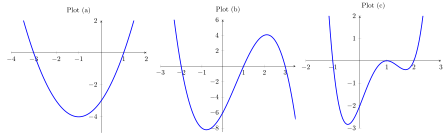
\includegraphics[width=0.99\columnwidth]{figures/0-6-fig5.pdf}
				\end{center}      
\end{activity}
\begin{smallhint}
How many roots are there and how do the ends behave?
\end{smallhint}
\begin{bighint}
    You may want to use Theorems \ref{T:0.6.1} and \ref{T:0.6.2} to determine the degree
    of the polynomial as well as the roots and factors.
\end{bighint}
\begin{activitySolution}
   \ba
        \item This function clearly has two roots and the ends show the same behavior.
            This indicates that this is likely a degree 2 polynomial (a quadratic).  Based
            on the roots $x=-2$ and $x=1$ the factors are $(x+2)$ and $(x-1)$ so the
            polynomial is of the form $a(x) = C(x+2)(x-1)$.  Finally, it appears that the
            point $(-1,-4)$ is on the curve so $C=2$ and the polynomial is 
            \[ a(x) = 2(x+2)(x-1). \]
        \item This function clearly has three roots and the ends show the opposite
            behavior.  Since the right-hand side of the function tends down we expect a
            negative leading coefficient.  Based on the roots $x=-2$, $x=1$, and $x=3$ the
            factors are $(x+2)$, $(x-1)$, and $(x-3)$ and the polynomial takes the form
            $b(x) = C(x+2)(x-1)(x-3)$.  The point $(-1,-8)$ appears to be on the graph so
            $C = -1$ and the polynomial is
            \[ b(x) = -(x+2)(x-1)(x-3). \]
        \item This function clearly has three roots but the end behavior indicates an even
            degree polynomial.  The root at $x=1$ is special since we do not cross the $x$
            axis.  Hence, the factors are $(x+1)$, $(x-1)$, $(x-1)$, and $(x-2)$.  Notice
            that the $(x-1)$ root is listed twice, and hence the polynomial takes the form
            $c(x) = C(x+1)(x-1)^2(x-2)$.  The point $(0,-2)$ appears to be on the graph so
            $C = 1$ and the polynomial is
            \[ c(x) = (x+1)(x-1)^2(x-2). \]
   \ea
\end{activitySolution}

\aftera

\newpage
\begin{activity}\label{A:0.6.3}
% The purpose of this activity is to prompt students to start thinking about vertical asymptotes (and division by 0) in terms of limits.  
\ba
		\item Suppose $f(x) = x^{2}+ 3x + 2$ and $g(x) = x - 3$.  
			\begin{enumerate}
                \item[(i)] What is the behavior of the function $h(x) = \displaystyle{\frac {f(x)}{g(x)}}$ near $x = -1$? (i.e. what happens to $h(x)$ as $x\to -1$?) near $x = -2$? near $x = 3$?
                \item[(ii)] What is the behavior of the function $k(x) = \displaystyle{\frac {g(x)}{f(x)}}$ near $x = -1$? near $x = -2$? near $x = 3$?
			\end{enumerate}
		\item Suppose $f(x) = x^{2} - 9$ and $g(x) = x - 3$.  
			\begin{enumerate}
                \item[(i)] What is the behavior of the function $h(x) = \displaystyle{\frac {f(x)}{g(x)}}$ near $x = -3$? (i.e. what happens to $h(x)$ as $x\to -3$?) near $x = 3$?
                \item[(ii)] What is the behavior of the function $k(x) = \displaystyle{\frac {g(x)}{f(x)}}$ near $x = -3$? near $x = 3$?
			\end{enumerate}
% 		\item Suppose $f(x) = \sin{x}$ and $g(x) = x$.
% 			\begin{enumerate}
%                 \item[(i)] What is $f(0)$? What is $g(0)$?
%                 \item[(ii)] What is the behavior of the function $h(x) = \displaystyle{\frac {f(x)}{g(x)}}$ near $x = 0$? (i.e. what happens to $h(x)$ as $x\to 0$?)
%                 \item[(iii)] What is the behavior of the function $k(x) = \displaystyle{\frac {g(x)}{f(x)}}$ near $x = 0$?
% 			\end{enumerate}
\ea

\end{activity}
\begin{smallhint}
    Watch carefully for division by zero.  That is where a vertical asymptote is possible.
\end{smallhint}
\begin{bighint}
    Watch carefully for division by zero.  That is where a vertical asymptote is possible.
\end{bighint}
\begin{activitySolution}
   \ba
        \item For $f(x) = x^2+3x+2$ and $g(x) = x-3$ when we form the function $h(x) =
            f(x)/g(x)$ we get $h(x) = \frac{x^2+3x+2}{x-3}$.  Notice that $h(-1) = 0$ and
            $h(-2) = 0$ since $f(-1) = f(-2) = 0$ and $g(-2) \neq 0$.  At $x=3$, on the
            other hand, $g(x) = 0$ and there is a vertical asymptote on the function
            $h(x)$.

            For $k(x) = g(x) / f(x)$.  The vertical asymptotes occur at $x=-2$ and $x=-1$
            and a zero occurs at $x=3$.
        \item For $f(x) = x^2-9$ and $g(x) = x-3$ we see immediately that $f(x)$ can be
            factored to $f(x) = (x-3)(x+3)$ and hence the function $h(x) = f(x)/g(x)$
            simplifies to $h(x) = x+3$ when $x$ is not $3$.  When $x=3$ there is a
            discontinuity in the graph but this is not a vertical asymptote since the
            discontinuity can be removed algebraically.

            For $k(x) = g(x)/f(x)$ we simplify to $k(x) = 1/(x+3)$ when $x$ is not $3$.
            Therefore there is a vertical asymptote at $x=-3$ and a removable
            discontinuity at $x=3$.
   \ea
\end{activitySolution}

\aftera

\newpage
\begin{activity}\label{A:0.6.4}

%The purpose of this activity is to encourage students to think of horizontal asymptotes in terms of "dominance" of the numerator over denominator (or vice versa).  
	
\ba
		\item Suppose $f(x) = x^{3} + 2x^{2}-x + 7$ and $g(x) = x^{2} + 4x + 2$.  
			\begin{enumerate}
				\item Which function dominates as $x \to \infty$?
				\item What is the behavior of the function $h(x) = \displaystyle{\frac {f(x)}{g(x)}}$ as $x \to \infty$?
				\item What is the behavior of the function $h(x) = \displaystyle{\frac {g(x)}{f(x)}}$ as $x \to \infty$?
			\end{enumerate}
		\item Suppose $f(x) = 2x^{4} - 5x^{3} + 8x^{2} - 3x - 1$ and $g(x) = 3x^{4} - 2x^{2} + 1$
			\begin{enumerate}
				\item Which function dominates as $x \to \infty$?
				\item What is the behavior of the function $h(x) = \displaystyle{\frac {f(x)}{g(x)}}$ as $x \to \infty$?
				\item What is the behavior of the function $h(x) = \displaystyle{\frac {g(x)}{f(x)}}$ as $x \to \infty$?
			\end{enumerate}
        \item Suppose $f(x) = e^{x}$ and $g(x) = x^{10}$.
			\begin{enumerate}
				\item Which function dominates as $x \to \infty$ as $x \to \infty$?
				\item What is the behavior of the function $h(x) = \displaystyle{\frac {f(x)}{g(x)}}$ as $x \to \infty$?
				\item What is the behavior of the function $h(x) = \displaystyle{\frac {g(x)}{f(x)}}$ as $x \to \infty$?
			\end{enumerate}
\ea

\end{activity}\aftera

\newpage
\begin{activity}\label{A:0.6.5}
	For each of the following functions, determine (1) whether the function has a horizontal asymptote, and (2) whether the function crosses its horizontal asymptote.
\ba
		\item $f(x)=\displaystyle{\frac {x+3}{5x-2}}$
		\item $g(x)=\displaystyle{\frac {x^{2}+2x-1}{x-1}}$
		\item $h(x)=\displaystyle{\frac {x+1}{x^{2}+2x-1}}$
\ea
\end{activity}
\begin{smallhint}
    A horizontal asymptote occurs where the function approaches a value  as $x\to\infty$.
    It is possible for a function to cross a horizontal asymptote.
\end{smallhint}
\begin{bighint}
    A horizontal asymptote occurs where the function approaches a value  as $x\to\infty$.
    It is possible for a function to cross a horizontal asymptote.
\end{bighint}
\begin{activitySolution}
   \ba
        \item For $f(x) = \frac{x+3}{5x-2}$ the degrees of the two polynomials are both $1$
            so the numerator and denominator grow at the same rate.  The horizontal
            asymptote will be the ratio of the coefficients: $f(x) \to
            \frac{1}{5}$ as $x \to \infty$.  The graph does not cross the horizontal
            asymptote.
        \item In this case where $g(x) = \frac{x^2+2x-1}{x-1}$ the degree of the numerator
            is larger than the degree of the denominator so $g(x) \to \infty$ as
            $x\to\infty$ and there is no horizontal asymptote.
        \item In this case where $h(x) = \frac{x+1}{x^2+2x-1}$ the degree of the
            denominator is larger than the degree of the numerator so $h(x) \to 0$ as $x
            \to \infty$.  Therefore, there is a horizontal asymptote at $y=0$.  Observe
            that $h(-1) = 0$ so the function's graph does indeed cross the horizontal
            asymptote.
   \ea
\end{activitySolution}

\aftera

\newpage
\subsection*{Voting Questions}
\renewcommand{\labelenumi}{\thesection.\arabic{enumi}}
\begin{enumerate}
        \input{clicker/SVC.01.06.005.tex}
        \teacher{\input{clicker/SVC.01.06.005C.tex}}
        \input{clicker/SVC.01.06.010.tex}
        \teacher{\input{clicker/SVC.01.06.010C.tex}}
        \input{clicker/SVC.01.06.020.tex}
        \teacher{\input{clicker/SVC.01.06.020C.tex}}
        \input{clicker/SVC.01.06.030.tex}
        \teacher{\input{clicker/SVC.01.06.030C.tex}}
        \input{clicker/SVC.01.06.035.tex}
        \teacher{\input{clicker/SVC.01.06.035C.tex}}
        \input{clicker/SVC.01.06.040.tex}
        \teacher{\input{clicker/SVC.01.06.040C.tex}}
        \input{clicker/SVC.01.06.050.tex}
        \teacher{\input{clicker/SVC.01.06.050C.tex}}
        \input{clicker/SVC.01.06.060.tex}
        \teacher{\input{clicker/SVC.01.06.060C.tex}}
        \input{clicker/SVC.01.06.065.tex}
        \teacher{\input{clicker/SVC.01.06.065C.tex}}
        \input{clicker/SVC.01.06.066.tex}
        \teacher{\input{clicker/SVC.01.06.066C.tex}}
        \input{clicker/SVC.01.06.070.tex}
        \teacher{\input{clicker/SVC.01.06.070C.tex}}
        \input{clicker/SVC.01.06.075.tex}
        \teacher{\input{clicker/SVC.01.06.075C.tex}}
        \input{clicker/SVC.01.06.080.tex}
        \teacher{\input{clicker/SVC.01.06.080C.tex}}
        \input{clicker/SVC.01.06.090.tex}
        \teacher{\input{clicker/SVC.01.06.090C.tex}}
        \input{clicker/SVC.01.06.100.tex}
        \teacher{\input{clicker/SVC.01.06.100C.tex}}
        \input{clicker/SVC.01.06.110.tex}
        \teacher{\input{clicker/SVC.01.06.110C.tex}}
        \input{clicker/SVC.01.06.120.tex}
        \teacher{\input{clicker/SVC.01.06.120C.tex}}
\end{enumerate}
\renewcommand{\labelenumi}{\arabic{enumi}}

\newpage

 % Pre Calc topics
% \include{1.chap} % Understanding the Derivative
% \include{2.chap} % Computing derivatives
% \include{3.chap} % Using Derivatives
% \include{4.chap} % The Definite Integral
% \include{5.chap} % Finding Antiderivatives and Evaluating Integrals
% \include{6.chap} % Using Definite Integrals
% \include{7.chap} % Differential Equations
% \include{8.chap} % Sequences and Series
% 
% \include{9.chap} % Sequences, Difference Equations, and Discrete Dynamical Systems
% \include{10.chap} % Introduction to Linear Algebra
% 
% 
% \nocite{HughesHallet}
% \nocite{principles}
% \nocite{Arney}
% \nocite{nonlinear}
% \nocite{Noonburg}
% \nocite{Lay}
% 
% \pagebreak
% \bibliographystyle{plain}
% \bibliography{CarrollCalculusBib}
% \pagebreak
% 
%  \appendix
%  \include{A.Appendices}
% 
% \backmatter
% 	 
% \printindex

\end{document}
